
% This is misnamed filename. We wanted this to be the inrtoduction to
% the idea of adaptive runtime system

\begin{frame}[fragile]
\frametitle{An Empowered Runtime System}

\begin{itemize}
\item Think now, based on the model so far, what the runtime system
  can do
\item It is free to migrate chares across processors, as and when it pleases
\item It is free to schedule the method invocations (including
  constructors) that are waiting in the Queue on a processor in any
  order it pelases
\item Automatic Instrumentation
\begin{itemize}
\item It schedules invocations: so it knows how long they take
\item It mediates communication: so it knows which chares talk to whom
\end{itemize}

\end{itemize}

\end{frame}

\begin{frame}[fragile]
\frametitle{An Introspecitve and Adaptive Runtime System (CHANGE FIG)}
\begin{itemize}
\item Based on these capabilities, Charm++ runtime includes:
\begin{itemize}
\item Load balancing Schemes
\item Fault Tolerance Schemes
\item Communication optimizers
\end{itemize}
\end{itemize}

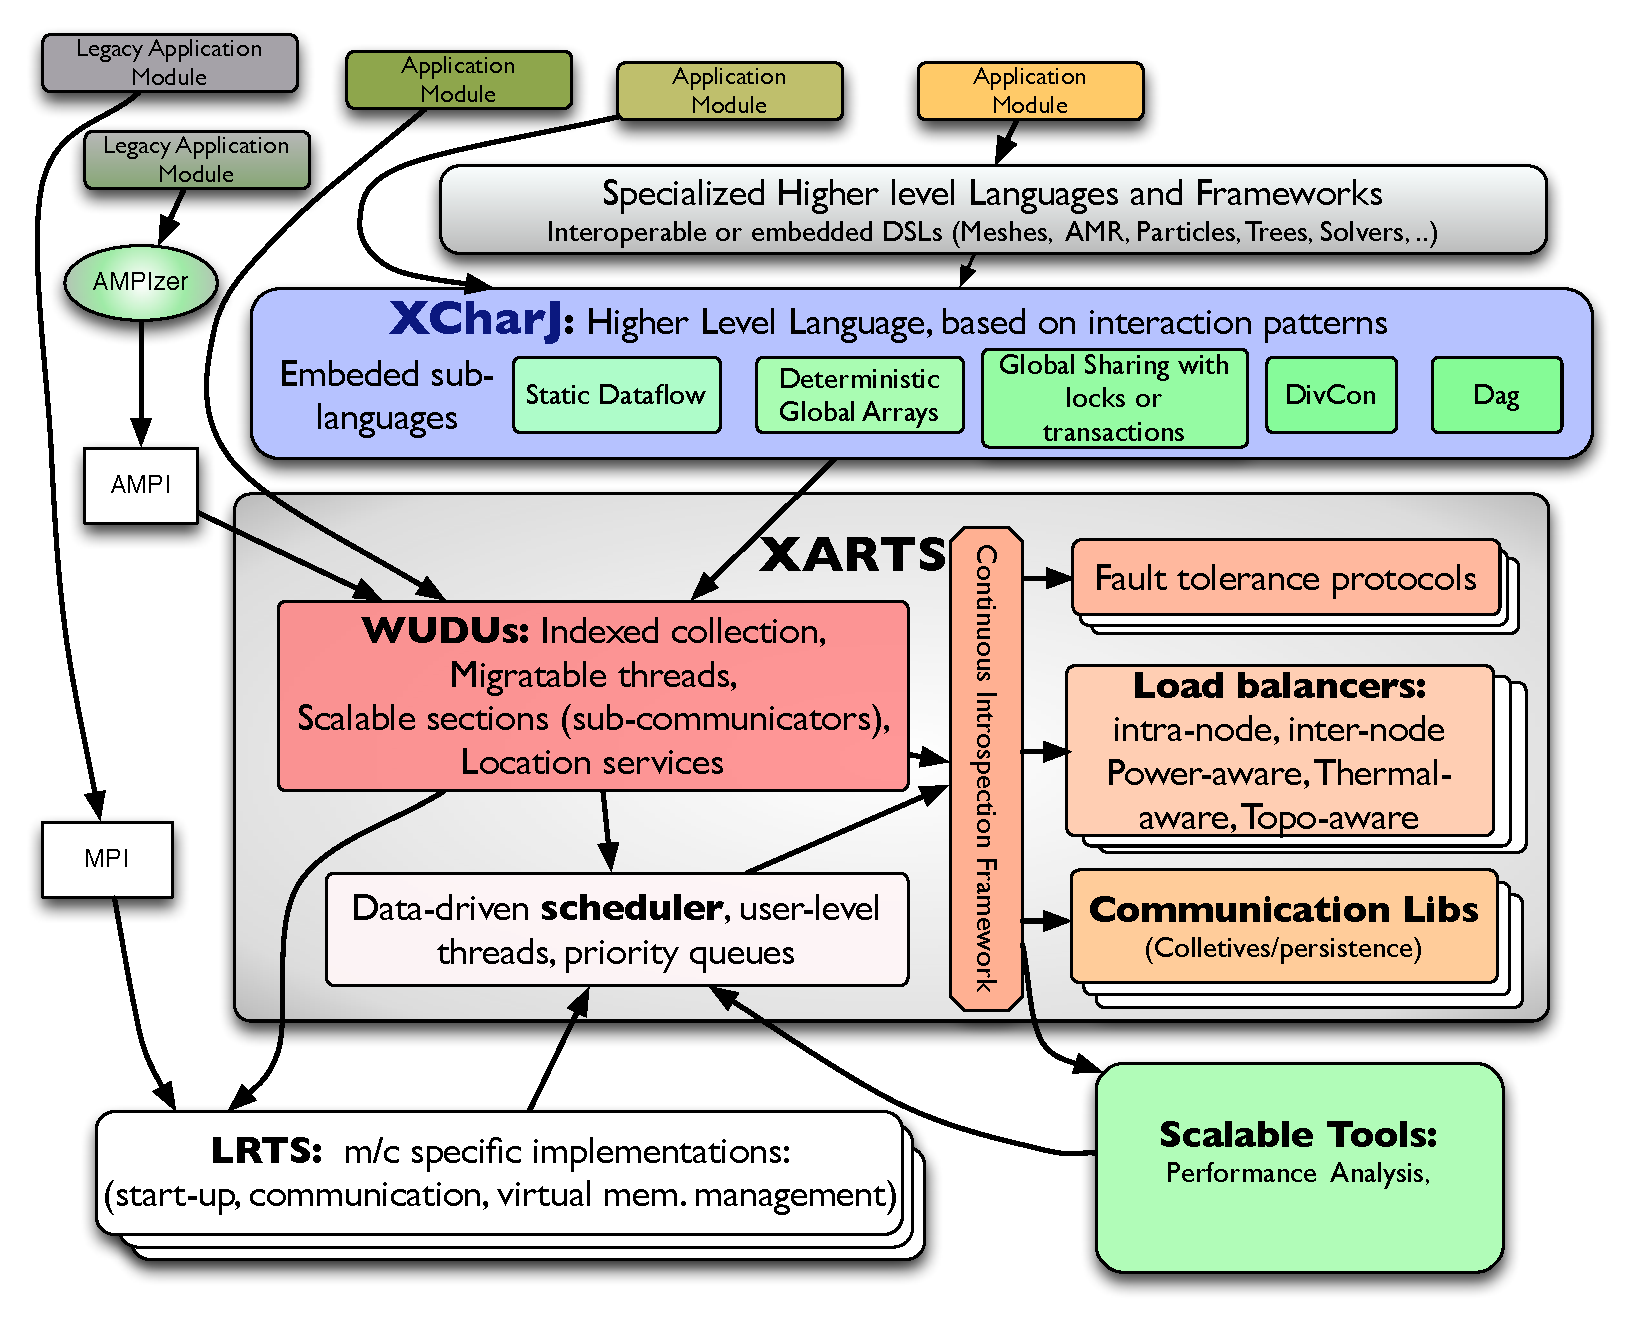
\includegraphics[width=0.8\textwidth]{figures/arts}

\end{frame}

